\documentclass[a4paper, 11pt]{article}
\usepackage{amsmath}
\usepackage{amsfonts}
\usepackage{amssymb}
\usepackage{caratula}
\usepackage[spanish, activeacute]{babel}
\usepackage[usenames,dvipsnames]{color}
\usepackage[width=15.5cm, left=3cm, top=2.5cm, height= 24.5cm]{geometry}
\usepackage{graphicx}
\usepackage[utf8]{inputenc}
\usepackage{listings}
\usepackage[all]{xy}
\usepackage{multicol}
\usepackage{subfig}

\usepackage{cancel}
\usepackage{float}
\usepackage{xcolor}
\usepackage{color,hyperref}

\usepackage{multirow} % para las tablas


%%%%%%%%%%%%%% ALGUNAS MACROS %%%%%%%%%%%%%%
% For \url{SOME_URL}, links SOME_URL to the url SOME_URL
\providecommand*\url[1]{\href{#1}{#1}}

% Same as above, but pretty-prints SOME_URL in teletype fixed-width font
\renewcommand*\url[1]{\href{#1}{\texttt{#1}}}

% Comando para poner el simbolo de Reales
\newcommand{\real}{\hbox{\bf R}}

\providecommand*\code[1]{\texttt{#1}}

%uso: \ponerGrafico{file}{caption}{scale}{label}
\newcommand{\ponerGrafico}[4]
{\begin{figure}[H]
	\centering
	\subfloat{\includegraphics[scale=#3]{#1}}
	\caption{#2} \label{fig:#4}
\end{figure}
}

%\renewcommand{\algorithmiccomment}[1]{\hfill #1}

%%%%%%%%%%%%%%%%%%%%%%%%%%%%%%%%%%%%%%%%%%%%

\materia{Ingeniería de Software II}

\titulo{Big Tiza}
%\fecha{fecha de entrega}
%\grupo{Nro grupo}
\integrante{Agustina Ciraco}{630/06}{agusciraco@gmail.com}
\integrante{Alejandro Rebecchi}{15/10}{alejandrorebecchi@gmail.com}
\integrante{Maria Lara Gauder}{27/10}{marialaraa@gmail.com}
\integrante{Martin Heredia}{146/11}{martin.herediaf@gmail.com}

\include{templates}

\begin{document}
\pagestyle{myheadings}
\maketitle
%\markboth{Nombre materia}{Nombre TP}

\thispagestyle{empty}
\tableofcontents

%\setcounter{section}{-1}
\newpage

\section{Introducci\'on}
En el Trabajo Práctico 1 se desarrolló e implementó un sistema llamado ''AULA al 2020'' que consiste en un sistema de alertas a los alumnos de una escuela mediante un SMS a sus celulares. Los Docentes y el personal de la Secretaría o Dirección comprendían el usuario del sistema, es decir, quienes creaban campañas y/o eventos, los mensajes para las mismas y al finalizar, cargaban los resultados obtenidos. Debido al gran éxito en la implementación del mismo para una escuela de Urquiza, se decide ampliar el programa para que permita campañas a nivel masivo. Ya no hablamos de una escuela, sino que intervienen munincipios, provincias y a nivel nacional. 

Se detallan, en primer lugar, los atributos de calidad junto con sus respectivos escenarios, deducidos a partir de la consigna y de la QAW realizada. 
Se presentan, entonces, las arquitecturas del sistema inicial (''AULA al 2020'') y la correspondiente al sistema pedido por el Ministro, cuyo alcance es a nivel nacional. Para esta última arquitectura, se trata de cumplir con los objetivos requeridos por el cliente. Por otro lado, se presenta una discusión sobre las diferencias entre las metodologías utilizadas en cada proyecto.


\newpage
\section{Atributos de Calidad}
\subsection{Listado atributos de calidad definidos}
\begin{itemize}

\item[Performance] \textit{No se acepta ningún tipo de demoras ante el monitoreo del estado de las campañas.}\\
\textbf{Fuente}: Externa. \\
\textbf{Estímulo}: El usuario desea ver el estado actual de la campaña. Requiere visualización de las estadísticas generadas hasta el momento, de los mensajes enviados y los no enviados. \\
\textbf{Entorno}: Normal.\\
\textbf{Artefacto}: Sistema.\\
\textbf{Respuesta}: Se procesa el pedido de visualizar el estado de la campaña.\\
\textbf{Medición de la respuesta}: El pedido debe resolverse en menos de un segundo. \\

\item[Disponibilidad] \textit{Se pueden generar fallas de comunicación durante la transición de servidores.}\\
\textbf{Fuente}: Interna.\\
\textbf{Estímulo}: Falla por omisión.\\
\textbf{Entorno}: Normal, el sistema funciona en su modo habitual.\\
\textbf{Artefacto}: Canal de comunicación.\\
\textbf{Respuesta}: Se deberá pasar a un entorno degradado, donde se solucionen los pedidos realizados durante la transición, sin importar la performance del sistema.\\
\textbf{Medición de la respuesta}:  Se permanecerá en modo degradado hasta que se termine la transicción.\\

\item[Modificabilidad] \textit{Cambio de servidores de etapa en Córdoba (ArSAT) a etapa país.}\\
\textbf{Fuente}: Administrador. \\
\textbf{Estímulo}: Se quiere aumentar la cantidad de servidores para poder almacenar datos de todos los usuarios del país. \\
\textbf{Entorno}: En ejecución. \\
\textbf{Artefacto}: Sistema. \\
\textbf{Respuesta}: Los nuevos servidores son agregados al sistema y ya estarán listos para ser usados. \\
\textbf{Medición de la respuesta}:  Tres horas.\\

\item[Seguridad] \textit{Un empleado de la munincipalidad no podrá ingresar a campañas creadas a nivel nacional por el gobernador de la provincia.}\\
\textbf{Fuente}: Usuario.\\
\textbf{Estímulo}: Intenta acceder al repositorio. \\
\textbf{Entorno}: Online \\
\textbf{Artefacto}: Sistema de almacenamiento. \\
\textbf{Respuesta}: Se le bloquea el acceso y, además, se registra el intento fallido de acceso. \\
\textbf{Medición de la respuesta}: La probabilidad de que una persona logre ingresar al sistema de almacenamiento es de 0,01\%. \\

\item[Seguridad] \textit{Se requiere almacenar todas las creaciones, modificaciones y accesos a los datos que se realicen. Por ejemplo, si el gobernador de Tierra del Fuego crea una campaña ''Contra el frío'', se debe registrar esa acción. }\\
\textbf{Fuente}: Usuario válido.\\
\textbf{Estímulo}: El usuario ingresa un nuevo dato a un repositorio.\\
\textbf{Entorno}: Control de accesos.\\
\textbf{Artefacto}: Repositorio.\\
\textbf{Respuesta}: Se almacena en otro repositorio el id del usuario, con la descripción del tipo de dato al que accedió y que tipo de acción realiza sobre el mismo.\\
\textbf{Medición de la respuesta}: Se registrarán todos los accesos.\\

\item[Disponibilidad] \textit{Falla de comunicación para el envío del mensaje a través del canal de comunicación normal en la provincia de Chubut.}\\
\textbf{Fuente}: Gestor de Mensajes. \\
\textbf{Estímulo}: Se intenta enviar un mensaje a un usuario en Chubut. \\
\textbf{Entorno}: Normal. \\
\textbf{Artefacto}: Sistema de env\'io de Mensajes. \\
\textbf{Respuesta}: El mensaje es enviado al usuario en cuesti\'on por medio del uso de los drones que replican la señal. Para lograrlo, se avisará de la necesidad a una empresa tercerizada encargada. \\
\textbf{Medición de la respuesta}: El mensaje a los habitantes de la provincia llega el 98\% de las veces. \\


\item[Certeza de Datos] \textit{El presidente actual del país quiere analizar los posibles resultados para todas las campañas a nivel nacional en actual funcionamiento.}\\
\textbf{Fuente}: Usuario. \\
\textbf{Estímulo}: Pide ver el estado actual de todas las campa\~nas. \\
\textbf{Entorno}: Normal. \\
\textbf{Artefacto}: Cliente resultados. \\
\textbf{Respuesta}: Se muestra por una interfaz un listado (de manera incremental) de todas las campa\~as con datos aproximados de sus estados actuales. \\
\textbf{Medición de la respuesta}: El 80\% del estado de las campa\~nas mostradas es correcto. \\

\item[Escalabilidad] \textit{Mantener la performance en el envío de mensajes
Se quiere expandir el sistema de la provincia de Córdoba a nivel nacional manteniendo la performance en el envio de mensajes.}\\
\textbf{Fuente}: Sistema. \\
\textbf{Estímulo}: Creación de una nueva campaña. \\
\textbf{Entorno}: Funcionamiento con 40 millones de posibles destinatarios para todos los mensajes. \\
\textbf{Artefacto}: Sistema de envío. \\
\textbf{Respuesta}: No se realiza ninguna modificación en el sistema, ya que el mismo ya se encuentra preparado para soportar los nuevos volúmenes de datos. \\
\textbf{Medición de la respuesta}: El tiempo de envío de mensajes aumenta en menos de un 10\%.\\

\item[Modificabilidad] \textit{A futuro se quiere poder permitir a empresas privadas crear campañas de promoción de productos.}\\
\textbf{Fuente}: Representantes de una empresa privada. \\
\textbf{Estímulo}: Carga de campaña. \\
\textbf{Entorno}: Normal. \\
\textbf{Artefacto}: Aplicación web. \\
\textbf{Respuesta}: Se adapta la aplicación para permitir la carga de campañas privadas de productos, con el agregado de todos los permisos que se requieran. \\
\textbf{Medición de la respuesta}: En menos de 2 semanas se deben hacer los cambios y poner en producción la nueva funcionalidad para la carga de campañas por empresas privadas. \\

\item[Flexibilidad] \textit{Permitir que diferentes proveedores de contenido adapten campañas nacionales a las condiciones locales de cada region.} \\
\textbf{Fuente}:  Proveedor de contenido.  \\
\textbf{Estímulo}: Adaptación de campaña. \\
\textbf{Entorno}: Funcionamiento normal. \\
\textbf{Artefacto}: Aplicacion web. \\
\textbf{Respuesta}: Se adapta la campaña a las condiciones de la región. \\
\textbf{Medición de la respuesta}: Se adapta la campaña en tiempo de ejecución ( sin necesidad de bajar el servidor o detener la aplicación ). \\

\item[Usabilidad] \textit{Se desea que los usuarios puedan crear campañas correctamente de forma fácil y rápida.} \\
\textbf{Fuente}:  Usuario. \\
\textbf{Estímulo}: Pedido de creación de campaña. \\
\textbf{Entorno}: Funcionamiento normal. \\
\textbf{Artefacto}: Aplicación web. \\
\textbf{Respuesta}: El usuario crea una campaña correctamente. \\
\textbf{Medición de la respuesta}: En un test de usabilidad el 95\% de los usuarios logra crear una campaña correctamente en menos de 5 minutos. \\

\item[Usabilidad] \textit{Se desea poder ver toda la información referida a una campaña de forma clara.} \\
\textbf{Fuente}:  Usuario. \\
\textbf{Estímulo}: Pedido de visualizacion de campaña. \\
\textbf{Entorno}: Funcionamiento normal. \\
\textbf{Artefacto}: Aplicación web. \\
\textbf{Respuesta}: Se visualiza toda la información disponible relacionada con la campaña. \\
\textbf{Medición de la respuesta}: En un test de usabilidad el 95\% de los usuarios logran extraer la información esperada en menos de 30 segundos. \\

\item[Usabilidad] \textit{Se desea poder comparar resultados de varias campañas de forma comparable, fácil de entender.} \\
\textbf{Fuente}: Usuario. \\
\textbf{Estímulo}: Pedido de comparación de resultados de 2 campañas. \\
\textbf{Entorno}: Funcionamiento normal. \\
\textbf{Artefacto}: Aplicacion web. \\
\textbf{Respuesta}: Se muestran los resultados de ambas campañas en la misma pantalla. \\
\textbf{Medición de la respuesta}: En un test de usabilidad el 95\% de los usuarios logran comprender los resultados en menos de 5 minutos. \\

\end{itemize}

\newpage

\section{Arquitecturas}
\subsection{Arquitectura TP1}
A partir del proyecto Aula al 2020, de los objetivos planteados y el prototipo desarrollado, se define el siguiente diagrama de arquitectura:

\centerline{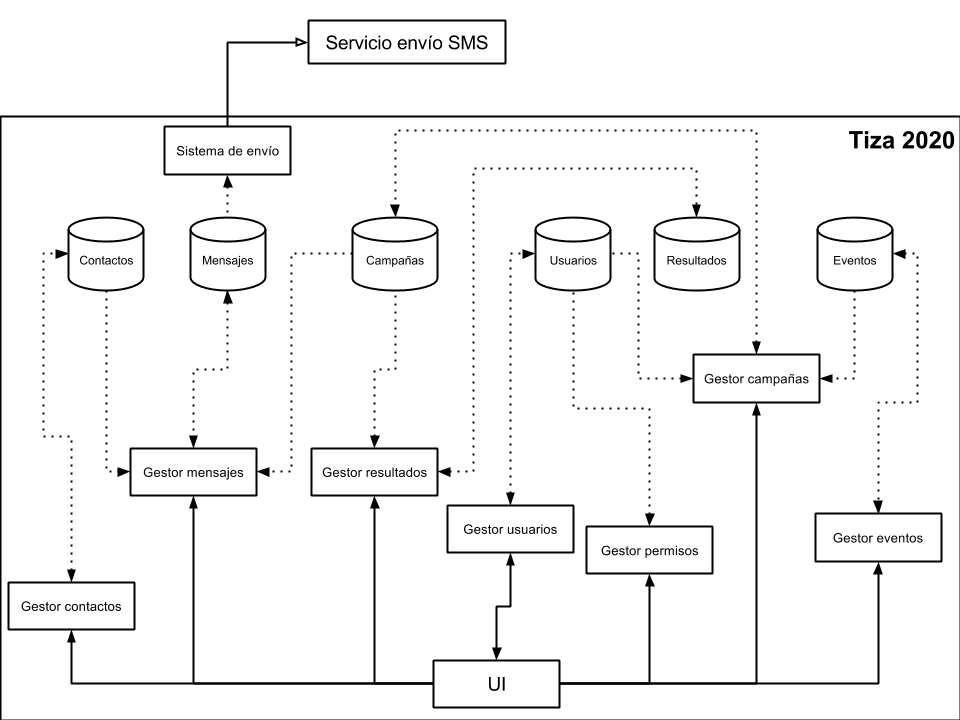
\includegraphics[width=1\textwidth]{./diagramas/ArquitecturaTP1.png}}
\centerline{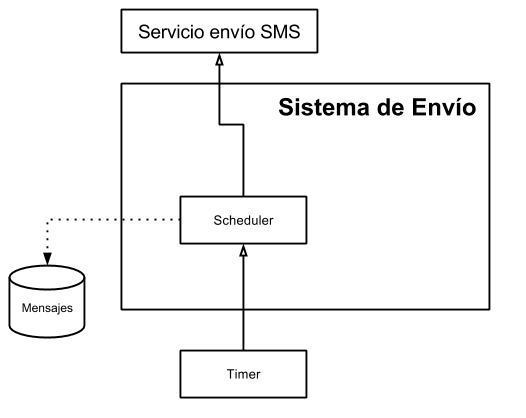
\includegraphics[width=0.4\textwidth]{./diagramas/ArqTP1SistEnvio.png}}

En primer lugar se presenta la UI, que es la encargada de la interacción del usario con el sistema de ''Tiza 2020''. La misma recibe los pedidos por parte del usuario. Para comenzar, se deberá validar el acceso del mismo, es decir, verificar su previa inscripción en el sistema. Para eso el UI indica al \textbf{Gestor usuarios} el id del usuario que intenta acceder. Este último lee la base de datos, buscando los datos del mismo. En caso de no existir, retorna al UI un aviso de usuario inválido, el cual se encargará de notificarle a la persona. Caso contrario, responde que se permite el acceso al usuario al sistema. 
En caso de que el usuario sea válido, el UI envía un pedido al \textbf{Gestor campañas}, pidiendo las campañas correspondientes al usuario para poder mostrarlas como el siguiente menú, luego del inicio de sesión. El componente \textbf{Gestor campañas}, pide del repositorio las campañas que tienen en el campo de \emph{usuario con permiso de acceso} al id del usuario. Luego, envía la información de todas las campañas, completándolo con los datos requeridos en los demás repositorios, como podría ser el caso de los teléfonos de los contactos. 
El proceso se repite para cada menú que el usuario desee ver. Además, el gestor se encargará de recolectar la información necesaria y traducirla a una interfaz para que sea comprensible por el usuario y se le enviará al UI, quien se encarga de mostarla. En el caso de de que se desee mostrar la agenda correspondiente a un usuario, para poder incluirlo en la creación de un mensaje, el UI pedirá al \textbf{Gestor contactos}, la información necesaria. Este último se encargará de acceder a la base de datos y recolecctar los datos pedidos. El proceso es el mismo para el \textbf{Gestor mensajes}, \textbf{Gestor resultados}, \textbf{Gestor eventos}, siendo cada uno el encargado de interpretar para el UI los datos necesarios y de armar la interfaz necesaria. 

Por otro lado, cuando un usuario, tanto Docente como personal de la Secretaría o Dirección, desean crear o modificar algún objeto del sistema, lo indicarán al UI, utilizando los accesos que correspondan, y este se encargará de avisar al gestor que corresponda con el objeto. El gestor correspondiente se encargará de agregar el nuevo objeto al repositorio necesario.  En caso de que se desee modificar uno existente, también levantará de la base de datos el objeto, le aplicará la modificación indicada por el usuario y lo volverá a cargar en el repositorio. 

El \textbf{Sistema de envío} es el encargado de enviar los mensajes. El \emph{Timer} le envía cada hora un mensaje asincrónico al \emph{Scheduler} con la hora y fecha actuales. El \emph{Scheduler} se encargará de leer en la base de datos aquellos menajes que cumplan con esa hora y fecha de envío. Al obtener todos los mensajes, los traducirá para poder ser interpretados por el \textbf{Servicio envío SMS}. Este último es un sistema externo que se contratará para cumplir la función de enviar los SMS necesarios. 

\newpage
\subsection{Arquitectura TP2}
\subsubsection{Vista Componentes y conectores}
La arquitectura de esta parte se realizó contemplando los atributos de calidad nombrados en la sección anterior. A continuación se muestra el diseño realizado para esta parte, seguido de un detalle de desiciones tomadas.

\centerline{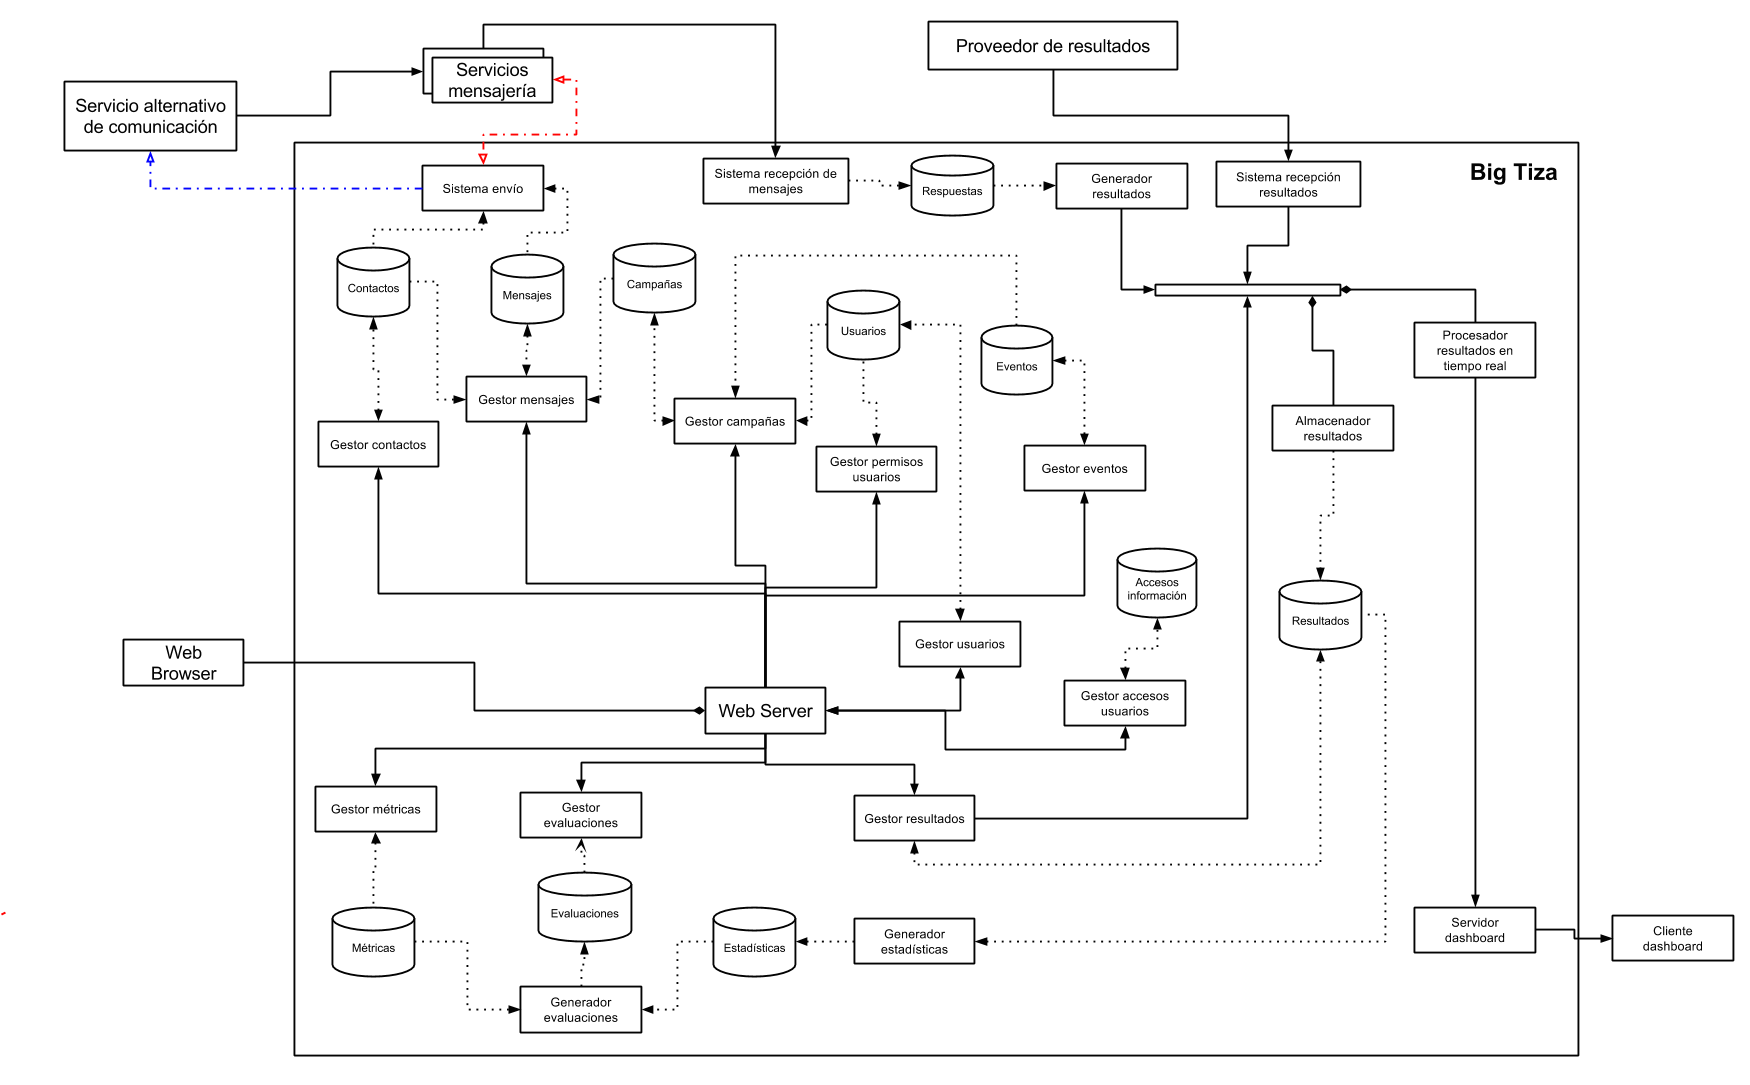
\includegraphics[width=1.2\textwidth]{./diagramas/VistaCompyCon.png}}
\centerline{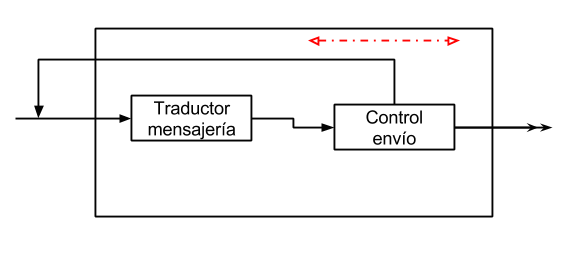
\includegraphics[width=0.5\textwidth]{./diagramas/ArqTP2Envio.png}}

Al momento de contemplar el atributo de calidad de \underline{Disponibilidad} respecto el envío de mensajes, se tomó la decisión de realizar la conexión entre componente \textbf{Servicios mensajería} y el componente \textbf{Sistema envío}, mediante dos conectores distintos. Dado que se tiene en cuenta que al momento de enviar mensajes, puede fallar la conexión con los distintos servicios (Twitter, Facebook, SMS). 
Se optó por crear dos conectores para esta unión, uno que muestra la conexión normal, sin fallas, y otro, la conexión considerando falla de comunicación.\\

\centerline{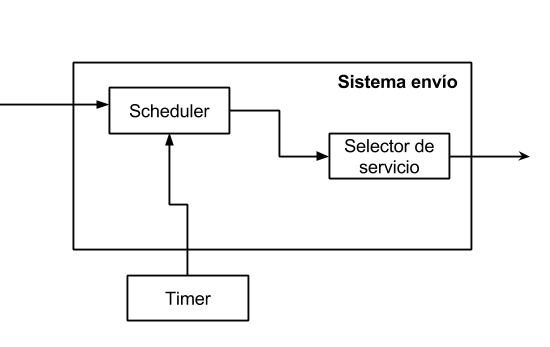
\includegraphics[width=0.5\textwidth]{./diagramas/ArqTP2conector1.png}}
\centerline{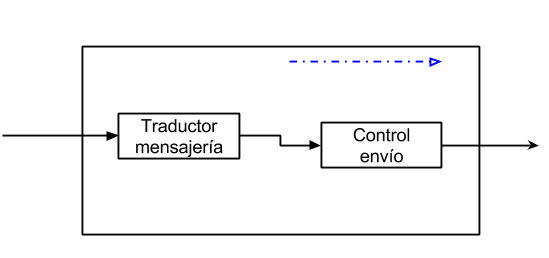
\includegraphics[width=0.5\textwidth]{./diagramas/ArqTP2conector2.png}}

Viendo en detalle el conector rojo, correspondiente al camino con posibles fallas, se puede observar que existe un traductor para poder comunicarse con cada tipo de servicio (Facebook, Twiter etc) ya que cada uno tiene un formato distinto.
En el caso del conector azul, de camino alternativo antes sucesivas fallas en el anteriormente descripto, se puede observar que se tiene el componente \textbf{Servicio alternativo de comunicación}, quién se encarga de tomar la decisión correspondiente, y realizar el envío de una forma tal que se cumpla el mismo (por ejemplo, mediante la repetición de la señal con drones).\\

%revisar que decision tomamos respecto a la version de oca
%Además, se contempló un tercer caso que coincide con el análisis de riesgo tomado para la parte de planificación del proyecto, donde se considera una conexión directa con un servicio de correo (OCA, por ejemplo), para poder contar con él en el caso de no tener ningún tipo de conexión con los otros servicios. No se observa este comportamiento en la arquitectora, ya que ese caso deberá ser resuelto manualmente por el usuario, ya que deja de poder solucionarse mediante el uso de software. \\ %de esa manera se desliga el sistema Big tiza de esa responsabilidad.

Es pedido por parte de los stakenholder que se recurra en lo menos posible al envío de la mensajería utilizando la empresa privada, por lo cual se prioriza un alto número de intentos de envío del mensaje a través del camino directo. En caso de que el sistema de comunicación continúe fallando, entonces ahí se recurrirá a caminos alternativos. \\
%Al considerar las situaciones de envío de camino sin fallas, donde como hay que evitar el uso de la empresa de telefonía privada, ya que esta puede generarle costos a los receptores, lo cual se desea evitar, por lo que se van a hacer varios intentos, antes de tomar la Decisión de cambiar de conector.\\

%~ Para la decision de por donde enviar se la asigna a un componente dentro de componente de envio de mensajes, esto se pude observar al hacer zoom de este comp 
Al momento de contemplar las acciones por parte de aquellas campañas que esperan respuestas a los mensajes enviados, se asume que los mismos seran enviados con un código para vincular con dicha campaña. En otras palabras, al enviarse un mensaje, sin importar su tipo, pero que espera respuesta por parte del usuario, se le asignará un número de identificación correspondiente a su campaña. El usuario al responder dará ese mismi id, que servirá para poder almacenar la respuesta de manera correcta en el sistema. El mensaje devuelto será recibido por el componente \textbf{Sistema recepción de mensajes}, que se encargará de almacenar el nuevo resultado en el repositorio correspondiente. El \textbf{Gestor resultados} traducirá las respuestas en resultados, para ser luego procesados. \\

Por otro lado, se tiene conexión con un sistema externo, denominado \textbf{Proveedor de resultados}, quien brinda resultados de encuestas realizadas para una determinada campaña. El tipo de resultado brindado irá variando de acuerdo al tipo de evaluación que desee hacer el usuario sobre una campaña. \\

Hasta el momento se mencionaron dos tipos diferentes de almacenamiento de los resultados, es decir, mediante un sistema externo o a partir de la respuesta de los mensajes por parte del usuario final. 
Además existe la situación de carga manual de resultados, que puede ser requerido, por ejemplo en el siguiente caso: en una campaña de vacunación, donde el efecto es que la persona se vacune y, cuando lo haga, eso suma un resultado a la campaña que será agregado al sistema por personal reponsable. 
Respecto a la arquitectura considerada para este punto, es contemplada en el componente \textbf{Gestor de resultados}, que es quien recibe los resultados cargados por una persona.\\

%Por otro lado, se contemplan campañas interactivas, es decir que envían mensajes cuyo efecto es una respuesta el mensaje envíado, por lo cual este tipo de resultados, se reciben directamente en el sistema, el encargado de recibirlo nuevamente es el componente gestor de resultados.\\

El procesamiento de resultados de las campañas se divide en dos ramas diferentes, la del almacenamiento directo de los mismos y la de visualización directa. 
Al recibir un resultado de una campaña, éste debe ser procesado inmediatamente para poder ser visualizado lo antes posible y así poder mantener un seguimiento en tiempo real de la campaña. Para poder cumplir con ese objetivo, el \textbf{Procesador de resultados en tiempo real} traduce los resultados para enviarlos al \textbf{Servidor dashboard}. El dashboard contempla el requerimiento de que las campañas se puedan monitorear de manera ágil. % El funcionamiento del mismo puede comprenderse a través de un ejemplo: se obtiene el resultado de que 4 personas recibieron la vacuna contra la gripe en el hospital Posadas, y a partir de las métricas definidas para la campaña  de ''Prevención de la gripe'', este valor dará un porcentaje de eficiencia. Es decir, cuanto progreso se obtuvo a partir de la aplicación de un campaña. Luego de evaluar dicho resultado, el mismo está listo para ser visualizado en el dashboard.\\
Por otro lado, todos los resultados en crudo serán almacenados, para poder ser evaluados, luego, y así generarse estadísticas finales. 
En este caso, el procedimiento será más lento, ya que se utilizará al finalizarse la ejecución de la campaña. En caso de querer observarse la eficiencia de la campaña en tiempo real, se podrá obtener la aproximación en el dashboard. 
Se tomó esta decisión teniendo en cuenta el volumen de información a procesar y los recursos con los que se cuentan. Durante la vigencia de una campaña se van a obtener volúmenes muy grandes de resultados parciales y como es pedido que se observe en tiempo real la influencia de una campaña, se debió recurrir a un nuevo sistema de procesamiento.\\

Otro aspecto que fue considerado al momento de definir la interfaz, es el de \underline{Seguridad}, ya que se hizo hincapié en que van a haber distintos tipos de usuario, y cada uno tendrá restricciones sobre la información. Es sumamente importante este tipo de restricciones, para cuando en un futuro se quiera agregar a empresas privadas en el sistema. Las mismas deberán tener un mínimo acceso a la información de campañas y ningún acceso a las campañas ajenas. A partir de un Web Server se controla los permisos de accesos a los usuarios. El Web Server pregunta al \textbf{Gestor de usuarios} si es correcto el intento de acceso por parte de un usuario. El gestor buscará en el repositorio \textbf{Usuarios} al usuario y retornará lo que corresponda. \\

Otras consideraciones que se tienen respecto a la seguridad de la información, es que los otros canales de acceso al sistema, como por ejemplo, la carga de resultados o dentro del componente \textbf{Sistema recepción de mensajes}, tengan revisiones de seguridad previo al intento de acceso a la base de datos por parte de un usuaria. De esta manera se persiste información evitandose así un potencial ataque de seguridad.\\

\newpage
\subsubsection{Vista Alocación}

\centerline{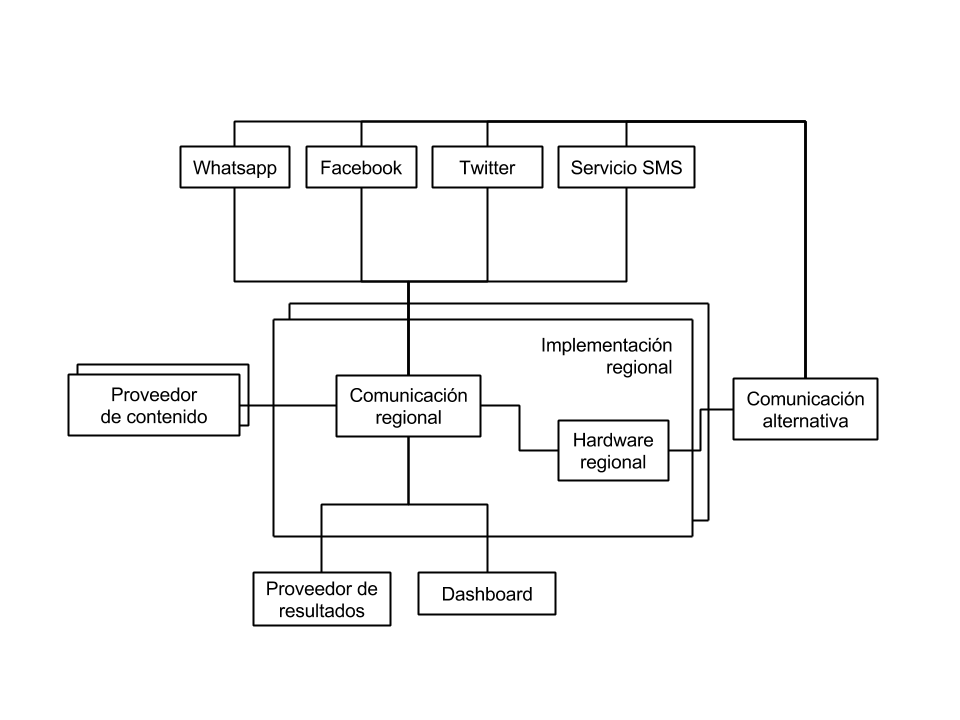
\includegraphics[width=0.8\textwidth]{./diagramas/VistaAlocacion.png}}

En esta vista se muestran donde está contenido cada componente externo presentado en la vista anterior. En este diagrama se puede observar que los servicios de mensajería se separan y muestran cada uno en particular. Se considera que cada servicio corre por separado ya que son empresas diferentes y presentan comportamientos distintos.\\

Por otro lado el \textbf{Proveedor de contenido} es aquel componente responsable de agregar a las campañas aquellos logos, mensajes o lo que se desee mostrar al usuario final. Esto se decidió en consideración a que las campañas van a ser de distintas índoles, ya sea para creación de una por el Ministerio de Salud, como por el Ministerio de Seguridad Vial, y en particular en un futuro se consideran las campañas de empresas privadas.\\

El \textbf{Proveedor de resultados} corresponde a un sistema externo encargado de enviar aquellos resultados que obtenga de las campañas y que desee sumar al momento de generar las estadísticas de las mismas. \\

El \textbf{Dashboard} es encargado de mostrar en tiempo real, estadísticas parciales realizadas de las distintas campañas. \\

Por último, se puede destacar el componente \textbf{Comunicación alternativa}, a quien se le asigna en el conector que ocurre cuando hay falta de conexión por el sistema normal. El sistema Big Tiza delegará esta tarera a una empresa tercerizada cuando esto ocurra. \\

Se observa que la vista de la sección anterior, es representada acá como una \textbf{Implementación regional}. Eso se debe a que el sistema de Big Tiza es replicado en diversos servidores para poder tener alcance nacional. En el caso de la provincia de Córdoba y algunas cercanas, tendrán el sistema cargado en los dos servidores ofrecidos por ArSAT, mientras que el resto se encontrará en sistemas externos privados. \\


%~ \subsection{Discusión de Arquitecturas}
\newpage
\subsection{Programming in the Large vs Programming in the Small}

En esta secci\'on se comparar\'an la Arquitectura correspondiente al Dise\~no Orientado a Objetos (small programming) y la nueva Arquitectura de gran escala (large programming) correspondientes a este trabajo.

{\bf Comunicaciones con entidades externas} \\
\begin{tabular}{| p{8cm} | p{8cm} |}
\hline
Dise\~no O. O. & Arquitectura \\ \hline \hline
Un solo componente externo, correspondiente al Sitema de Env\'io de Mensajes. Esto se debi\'o a que era el \'unico canal de comunicaci\'on. Con respecto a los resultados, estos eran cargados manualmente al sistema. & La cantidad de canales de comunicaci\'on aumentaron, no s\'olo abarcando al anterior Sistema de Envio de Mensajes, sino tambi\'en a redes sociales como Facebook y Twitter, y la posibilidad de env\'io por Correo Argentino. Para los resultados, como la cantidad de mensajes y respuestas son masivas, hacerlo manualmente ser\'ia imposible. Para esto se cuenta con la opci\'on de poder ser cargadas autom\'aticamente por medio de Web Services externos (como por ejemplo, un Web Service ofrecido por el Ministerio de Salud, para obtener resultados de campa\~nas de salud) \\ \hline
\end{tabular}


{\bf Seguridad de datos} \\
\begin{tabular}{| p{8cm} | p{8cm} |}
\hline
Dise\~no O. O. & Arquitectura \\ \hline \hline

La comunicaci\'on con el sevicio de Mensajer\'ia SMS era insegura. Cualquier persona podr\'ia capturar el tr\'afico y obtener datos privados de los usuarios. & Ahora nuestro sistema al ser a escala Provincial (y posteriormente a escala Nacional), debe garantizar la seguridad de los datos de cada usuario. Esto se logra por medio de algortimos de encriptaci\'on. \\ \hline
\end{tabular}


{\bf Disponibilidad} \\
\begin{tabular}{| p{8cm} | p{8cm} |}
\hline
Dise\~no O. O. & Arquitectura \\ \hline \hline

No siempre estaba garantizado que los mensajes enviados efectivamente llegaran. Si luego de 3 intentos no se lograba enviar algun mensaje, se lo descartaba. & Para intentar suplir la anterior falla, los mensajes persisten en el tiempo, y mientras tenga sentido el mensaje en el contexto de su campa\~na y a\'un no haya llegado, se prueba el env\'io por otros medios previamente mencionados o se reenintenta en caso de haber ya agotado todos los canales posibles. \\ \hline
\end{tabular}

{\bf Alocaci\'on} \\
\begin{tabular}{| p{8cm} | p{8cm} |}
\hline
Dise\~no O. O. & Arquitectura \\ \hline \hline

Al no ser muy grande el sistema y la cantidad de datos no era demasiada, con una m\'aquina alcanzaba para alocar cada componente del mismo y almacenar las campa\~nas, mensajes, usuarios y destinatarios. & Ahora aparece el conceto de BigData. Se cuenta con una masiva cantidad de datos y a la vez est\'a la necesidad de implementar sistemas performante. Es por esto que ahora el sistema esta alocado en varios servidores, aprovechando la capacidad de paralelizar trabajo y distribuir estrat\'egimante los datos entre todos estos lugares. \\ \hline
\end{tabular}


{\bf T\'acticas} \\
\begin{tabular}{| p{8cm} | p{8cm} |}
\hline
Dise\~no O. O. & Arquitectura \\ \hline \hline

En esta arquitectura no se ven reflejadas ninguna de las t\'acticas de atributos de calidad, ya que no fueron tenidas en cuenta. & Se vi\'o en la necesidad de aplicaci\'on de algunas t\'acticas para la resoluci\'on de problemas t\'ipicos de Disponibilidad, Performance, Seguridad entre otros. \\ \hline
\end{tabular}


{\bf Big Data} \\
\begin{tabular}{| p{8cm} | p{8cm} |}
\hline
Dise\~no O. O. & Arquitectura \\ \hline \hline

Como se mencion\'o previamente, en esta etapa la cantidad de datos es m\'inima, con lo cual esto permit\'ia que para poder obtener el estado de todas las campa\~nas, con un simple listado de las mismas se lograba visualizarlas, y no se consum\'ia mucho tiempo. & En cambio, y como tambi\'en se mencion\'o, en esta etapa al haber una inmensa cantidad de datos, la visualizaci\'on de las campa\~nas pasa a ser un reto. Aparece la necesidad de aplicar heur\'isticas usando estad\'isticas para dar una idea del estado de las mismas, debido a la imposibilidad de brindar un servicio exacto tiempo real. \\ \hline
\end{tabular}

\newpage

\section{Discusi\'on}

\subsection{Agile vs UP}

El proceso de desarrollo de la aplicación se separó en dos etapas. En la primera, cuando se pensaba una aplicación de pequeña escala, se trabajó con metodologías ágiles, específicamente con SCRUM. Ésta propone realizar un proceso iterativo incremental separado en sprints cortos (generalmente menos de dos semanas), flexible, adaptable, manejando como unidad de trabajo user stories y sus tareas. Al inicio del proceso se cargan en el backlog todas las user stories asignandoles un esfuerzo y un valor para el cliente. Luego al inicial cada sprint se eligen entre las pendientes, las que tienen la mejor relación valor/esfuerzo. Esto tiene algunos problemas, ya que no permite ver con mucha claridad el estado actual del proyecto o proyecciones a futuro. Se centra principalmente en el sprint actual.

Por otro lado, en la segunda etapa, en la que se pensaba una aplicación de gran escala y se trabajo baja la modalidad de UP (proceso unificado), la cual propone un proceso también iterativo incremental, pero organizado en fases(inicio, elaboración, construccion y transicion), compuestas por iteraciones. Al iniciar, de forma similar a SCRUM, se definen todos los casos de uso, pero luego se asignan directamente a iteraciones, y éstas a su vez a sus etapas correspondientes. De esta forma se tiene una visualización mas completa de todo el proceso, y durante el desarrollo del mismo, se puede tener una noción mas clara de la etapa actual y la proyección a futuro. A su vez ésto limita un poco la flexibilidad del esquema, requiriendo modificaciones en el plan ante eventuales retrasos u otro tipo de inconvenientes.

%\section{Discusión}

%\subsection{Agile vs UP}

El proceso de desarrollo de la aplicación se separó en dos etapas. En la primera, cuando se pensaba una aplicación de pequeña escala, se trabajó con metodologías ágiles, específicamente con SCRUM. Ésta propone realizar un proceso iterativo incremental separado en sprints cortos (generalmente menos de dos semanas), flexible, adaptable, manejando como unidad de trabajo user stories y sus tareas. Al inicio del proceso se cargan en el backlog todas las user stories asignandoles un esfuerzo y un valor para el cliente. Luego al inicial cada sprint se eligen entre las pendientes, las que tienen la mejor relación valor/esfuerzo. Esto tiene algunos problemas, ya que no permite ver con mucha claridad el estado actual del proyecto o proyecciones a futuro. Se centra principalmente en el sprint actual.

Por otro lado, en la segunda etapa, en la que se pensaba una aplicación de gran escala y se trabajo baja la modalidad de UP (proceso unificado), la cual propone un proceso también iterativo incremental, pero organizado en fases(inicio, elaboración, construccion y transicion), compuestas por iteraciones. Al iniciar, de forma similar a SCRUM, se definen todos los casos de uso, pero luego se asignan directamente a iteraciones, y éstas a su vez a sus etapas correspondientes. De esta forma se tiene una visualización mas completa de todo el proceso, y durante el desarrollo del mismo, se puede tener una noción mas clara de la etapa actual y la proyección a futuro. A su vez ésto limita un poco la flexibilidad del esquema, requiriendo modificaciones en el plan ante eventuales retrasos u otro tipo de inconvenientes.
%\subsection{Programming in the Large vs Programming in the Small}
En cuanto al desarrollo de la implementación del proyecto, dada la diferencia de magnitudes, para las distintas etapas utilizamos dos tipos de técnicas bastante diferentes. Para el primer caso, el de menor escala, utilizamos la técnica de programming in the small, la cual se centra en los detalles finos del diseño del modelo de datos del negocio. Se buscaespecìficamente que el código modele de forma semánticamente correcta las características de los objetos de interés del mundo real desde la perspectiva del negocio de interés.

Por su parte, para el segundo caso, el de mayor escala, se utilizó la técnica de programming in the large, la cual se centra en la arquitectura general del proyecto, sin hacer tanto incapié en detalles del código, sino que se manejan directamente modulos de código, componentes y conectores, e incluso componentes de hardware. Ésto nos brinda una visión más general del proyecto, mostrando su interacción con componentes externos y a su vez dando una visiòn más organizativa en general.

\newpage

\section{Conclusiones}

En este trabajo pr\'actico se compararon tanto arquitecturas como metodolog\'ias utilizadas para el primer trabajo pr\'actico de la materia con respecto a lo pedido en este trabajo.
En principio una de las grandes diferencias entre el trabajo pr\'actico 1 (de ahora en m\'as se refiere a este como TP1) con respecto a este, es el volumen de datos, usuarios y servicios de mensajer\'ia. Esto lleva a modelar de forma diferente cada sistema, ya que por ej\'emplo, en este trabajo, se tuvieron en cuenta a la hora de planificar y manejar tiempos, los riesgos, ya que es un proyecto a realizar en un plazo estimado de un a\~no. Por ello para evitar atrasos no contemplados, se trabaja en identificar riesgos y dependencias de tareas que puedan llevar a una demora indeseada. En cambio, en el TP1 al ser un proyecto de tan solo meses, se puede estimar con solo el dise\~no, aunque tambi\'en es una buena pr\'actica la identificaci\'on de dependencias de tareas.
Otra diferencia importante entre el TP1 y \'este es el manejo de Big Data. Esto se vio reflejado en la evaluaci\'on de resultados de campa\~nas, ya que en el TP1, dicha evaluaci\'on se realizaba en su totalidad y en poco tiempo. Sin embargo en el presente trabajo se trabajan con resultados parciales ya que el volumen de datos que se espera recibir es mucho mayor y eso implican demoras a la hora de evaluar la totalidad de datos. Como adem\'as se desea poder observar la campa\~na y tener lo m\'as actualizado posible el resultado, no se podr\'ia lograr esperando el resultado final.
En cuanto a las diferentes metodolog\'ias entre los trabajos mencionados, se not\'o que las metodolog\'ias aplicadas en el TP1 son m\'as din\'amicas ya que se manejan tiempos m\'as cortos, mientas que se notaron procesos m\'as largos en este trabajo, por lo comentado anteriormente en cuanto a, por ej\'emplo, planificaci\'on. Sin embargo, una similitud que se not\'o, aunque no se lleg\'o a aplicar, es que una vez definidas la planificaci\'on, arquitectura y se puede comenzar con el desarrollo del sistema de este trabajo pr\'actico, se pueden combinar metodolog\'ias de trabajo vistas en el TP1, como Scrum, y el manejo de Sprints.



\end{document}
